\chapter{Motivation and theoretical background}

The first section of this chapter lays the theoretical framework of the Standard Model (SM) of particle physics, including the historical discovery timeline of symmetries of nature, each corresponding to a leap forward in our physical understanding, and the model's particle content and their properties. The second section extends the symmetry group of the SM to include candidates for the observed cosmic dark matter (DM) and the particles that could mediate the DM-SM interactions.

\section{The Standard Model}

\subsection{Symmetries of nature}

Each major advance in the history of physics has corresponded to the discovery and mathematical implementation of a new global space-time, global discrete, or local gauge symmetry. In this section, I will review these discoveries, informally developing the mathematical framework needed to understand the symmetry groups of the SM. Along the way, two important subplots will play out: the development of our understanding of physics at smaller distance scales and higher energies, and the unification of previously separate physical sectors.

\indent Our ancient ancestors were aware that certain geometrical shapes, e.g. the Platonic solids, possessed the quality of symmetry, and were driven to understand the composition of physical substances by breaking them down into fundamental, indivisible units. These units, known as atoms by the ancient Greeks, interact and rearrange themselves according to physical laws to account for the variety of substances and physical phenomena we observe. The attraction to applying symmetry to nature is evidenced by the centuries-long belief that the Earth lie at the center of the universe, with the celestial bodies orbiting in perfect, divine circles.

\indent The end of the scientifically repressive middle ages brought along an improvement in astronomical observations and the growth of the pseudo-scientific field of alchemy, which attempted to reduce, understand, and manipulate the fundamental elements of physical substances. When Kepler discovered three laws of planetary motion, he unified the description of the motion of the planets. For the first time, the conservation of a physical quantity, what we now know as angular momentum, was associated with a general set of physical objects. At the burgeoning of the scientific revolution, Newton championed the idea that the same physical laws can be applied to all physical events, and that properties of these laws can be abstracted to apply to nature at a fundamental level.

\indent Newton defined an inertial reference frame implicitly as one where his first law held, that is, that an object remains at constant motion unless acted on by an outside force. Since his laws were the same in all inertial reference frames, a new symmetry of nature was discovered, now called symmetry under Euclidean transformations. Since Euclidean transformations form a mathematical group, it is said that classical mechanics is invariant under the Euclidean group. The invariance under the Euclidean transformations can be used to derive conservation laws: Newton's laws don't depend on spatial translations or rotations, implying the conservation of linear and angular momentum, respectively. These relationships foreshadow Noether's abstraction of the connection between continuous symmetries and conserved quantities. She proved that there is a conserved quantity, or current, associated with every symmetry of a physical system. This famous theorem facilitates the derivation of conserved quantities and will be used extensively in the theories that follow. The extension of the Euclidean transformations to include time translations and motion at constant velocity (boosts) forms the Galilean group.

\indent The next symmetry of nature to be discovered came when Lorentz found that Maxwell's equations, which unified the classical eletricity and magnetism sectors, were invariant under a set of transformations that generalized the classical Galiliean translations, now called Lorentz transformations, which form the Lorentz group. The Lorentz symmetry corresponds to the conservation law of total electric charge. Soon after, Einstein derived the Lorentz symmetry as a property of space-time itself through his special theory of relativity, assuming two simple postulates: the laws of physics and the speed of light are the same in all inertial reference frames. From these simple assumptions, Einstein was able to extend the classical laws of physics to the high velocity, high energy sector. Before Einstein, the symmetries of nature were thought to be consequences of the physical laws themselves, but Einstein's major paradigm shift was to view the symmetry itself as the more fundamental property, an insight key to his formulation of the general theory of relativity for the gravitational interaction. Combining the Lorentz and Euclidean transformations yields the Poincare group, the final global space-time symmetry of the SM.

\indent Just as relativists were probing physics at higher speeds and energies, other physicists were investigating the behavior of systems at smaller distance scales, conducting experiments to explore phenomena such as the Compton effect and photoelectric effect, which showed the quantized, particle-like behavior of light, and electron beam diffraction, which showed the wave-like behavior of electrons. Quantum theory was developed to consolidate the wave-like and particle-like behaviors of systems, and extended the validity of classical physics to microscopic scales. Where in classical physics particles states were described by their absolute position and momentum, quantum theory describes the state of a system by a probabalistic wavefunction. The classical symmetries and conservation laws carried over to quantum theory, with the concept of angular momentum generalized to include spin. Particles with zero or integer spin are called Bosons, and were shown to obey Bose-Einstein statistics, where the wavefunction is symmetric under all permutations of particles. Particles with half-integer spin, called Fermions, obey Fermi-Dirac statistics, where the wavefunction is symmetric under even permutations and changes sign under odd permutations, implying that no two particles can occupy the same state. These many-particle symmetries were applied to derive properties of materials and states of electrons in atomic and periodic systems, blackbody radiation, and many other properties of matter and radiation.

\indent Quantum theory was successfully applied to a myriad of low-energy systems. Dirac extended quantum theory and the Schrodinger equation, which describes the evolution of a quantum system in time, to the relativistic regime. His formulation of the wave equation for a spin-1/2 particle with mass m is inherently Lorentz invariant:

\begin{equation}
(i \gamma^\mu \partial_\mu - m)\psi = 0
\end{equation}

The solutions to the Dirac equation were found to have both positive and negative energy solutions, to the surprise of Dirac. His explanation was that the vacuum consisted of a "sea" of negative energy solutions, each in a distinct state due to the Pauli exclusion principle, and when a pair of electrons was produced, a positive energy state was filled and a negative energy state was vacated, creating a "hole" in the sea. The particle corresponding to this hole would have the same energy as the electron, but in order to conserve total charge, must have the opposite sign charge. This positively charged electron was not know to exist at the time, but was soon discovered in cosmic ray experiments and named the positron \cite{Bettini}. Dirac's theoretical prediction of the positron and its subsequent discovery opened the door for the discovery that every particle has an oppositely charged antimatter partner. 

\indent In an attempt to apply relativistic quantum theory to the electromagnetic field and the spin-0 photon, Dirac formulated the theory of quantum electrodynamics (QED) \cite{Dirac243}. QED is the first example of a quantum field theory (QFT), where the physical dynamics apply to the quantum field associated with a particle rather than the particle itself, and particles/antiparticles interact as excitations of the field. This formulation of creation and annihilation of particles and antiparticles gave a more physically intuitive explanation for the negative energy solutions of the Dirac equation than the Dirac sea. QED became the prototype for developing future relativistic quantum theories and Dirac's procedure the template for quantizing a general field theory. 

\indent With the discovery of antimatter and the apparatus of QFT in place, physicists continued searching for additional symmetries. If a particle state is an eigenvector of a symmetry operator, then the eigenvalue is an important quantum number of the state, since if the symmetry is conserved, the quantum number can be used to determine if a decay or interaction of this state is allowed \cite{}. Three important discrete symmetries operations, and their products, have had significant importance: space coordinate parity inversion (P), particle-antiparticle charge conjugation (C), and time reveral (T) \cite{Bettini}. P breaking observed by Wu, Yang, Lee, CP breaking obseved by Cronin, Fitch, PCT proved to be conserved symmetry \cite{}.

\indent The mid-20th century saw an explosion of discovery in particle physics and was a golden age for the feedback between theoretical and experimental work. The discovery of additional particles such as the muon \cite{}, pion \cite{}, neutrino\cite{}, and many others inspired the theoretical development of the quark model \cite{}, the refinement of QED \cite{}, and the formulation of theories to explain the strong \cite{} and weak \cite{} nuclear forces. Conversely, these new theories led to the prediction and subsequent discovery of new fundamental particles, such as the charm \cite{} and bottom \cite{} quarks, and composite particles, such as the $\Omega^-$ \cite{}.

\indent The development of the theories of the strong and weak forces unveiled a new set of symmetries: local invariance under unitary gauge transformations. In keeping with the trend of the discovery of new symmetries being associated with the unification of physical sectors, the electromagnetic and weak nuclear interactions were found to be components of a single force, called the electroweak force \cite{}. Again, with QED as the prototype, the Langrangians for the electroweak and strong forces were constructed to be invariant under unitary groups \cite{}. Early work by Weyl \cite{} showing the gauge invariance of electromagnetism was extended to QED, and lay the mathematical framework for describing the gauge invariance of the other forces. To demonstrate gauge invariance and how the gauge group generators are asssociated with the force carriers, take the QED terms of the SM Lagrangian as an example case:

\begin{equation}
\mathcal{L} \supset \bar{\psi} ( i \gamma^\mu D_\mu - m ) \psi - \frac{1}{4} F^{\mu\nu}F_{\mu\nu}
\end{equation}
where $A_\mu$ is the EM 4-potential and field corresponding to the photon, $F^{\mu\nu} = \partial^\mu A ^\nu - \partial^\nu A^\mu$ is the electromagnetic field tensor, and $D_\mu = \partial_\mu + i e A_\mu$ is the gauge covariant derivative. These terms are invariant under the the U(1) transformations

\begin{equation}
\psi \rightarrow e^{i\theta(x)} \psi.
\end{equation}

In general, the generators of an interaction's continuous symmetry group correspond to the gauge fields whose excitations are the gauge bosons that mediate that interaction. Just how $A_\mu$ is the field corresponding to the photon in QED and generator of the U(1) symmetry group of EM, the W and Z bosons and gluons are formed from the generators of the symmetry groups for the electroweak and strong interactions, SU(2)xU(1) and SU(3), respectively. Additionally, the covariant derivative is transformed in a way analagous to the QED covariant derivative, adding a factor for each generator with the corresponding charge in the coefficient. These charges (electric, color, weak isospin and hypercharge) are conserved for all of the forces in all interactions. The charges of the SM particles are described in more detail in the next section.

\indent Although the mathematical descriptions of their symmetries are similar, the EM, weak, and strong nuclear forces are quite different qualitatively. The EM force is the most familiar, being responsible for the interactions of matter and radiation at macroscopic scales, having only one type of charge which can be postitive or negative. The strong force is mediated by eight gluons, corresponding to the eight generators of SU(3), and carries three types of charge, known as red($R$), green($G$), and blue($B$). The "negatives" of these charges are called anticolors: antired($\bar{R}$), antigreen($\bar{G}$), and antiblue($\bar{B}$). Keeping with the visible color analogy, the theory of the strong force is called quantum chromodynamics (QCD). At low energies, the quarks and antiquarks are confined to form only color-neutral states. This is known as color confinement, and implies no free quarks exist, but only come in neutral combinations called hadrons. Since hadrons are strictly color-neutral, their states transform as the singlet representation under SU(3). At high energies, the strong coupling decreases, and the quarks can be treated as effectively free particles with perturbation theory using Feynman diagrams. This property of the strong force is known as asymptotic freedom. The weak force is qualitatively different than either the EM or strong forces, as particles do not exchange its mediators to form bound states of any kind. The low-energy limit of the weak theory was developed by Fermi to explain beta decays \cite{}, but the full description was not developed until the electroweak force was formulated. 

\indent The unification of the electromagnetic and weak interactions into the electroweak force at about 100 GeV had one major shortcoming: the invariance of the Lagrangian required the gauge bosons, $B$ from U(1) and $W^1, W^2, W^3$ from SU(2), to be massless. While the photon is indeed massless, the W and Z bosons have a nonzero mass \cite{}. Higgs and others \cite{} proposed a solution by introducing a new scalar field whose excitations were called the Higgs boson (H). The scalar field is a complex doublet, meaning it has four total real components, and its vacuum expectation value (vev), or value throughout all of space, is one of many non-zero values in the bottom of its "Mexican hat" potential. This spontaneous symmetry can be broken by choosing one of the values for the vev: $H = \frac{1}{\sqrt{2}} (0, \nu)$, where $\nu=246$ GeV is called the H vev. At energies above $O(100)$ GeV, the electroweak symmetry is obeyed, the gauge bosons are massless, and the Higgs field has one of many values along the circle at the base of its potential. When the H field is expressed as a perturbation about this vev, the electroweak symmetry is broken into the weak and EM forces, and mass terms are generated for the weak force bosons, which are expressed as linear combinations of $B, W^1, W^1, W^3$. The process of the Higgs acquiring a vev, spontaneously breaking the symmetry in its potential, and generating the masses of the weak bosons, is know as the Higgs mechanism, and results in the breaking of the electroweak symmetry. This mechanism can be carried out for a general operator depending on H with the substitution

\begin{equation}
H \rightarrow \frac{1}{2} (\nu + h)
\end{equation}
where $h$ is the physical Higgs, corresponding to the leftover degree of freedom of the H doublet that is not absorbed by the three massive gauge bosons. H couples to the SM fermions, detailed in the next section, not by the same mixing as described for the gauge bosons, but via Yukawa interactions, direct couplings whose coefficients are related the the fermion masses. The Higgs mechanism was the final piece of the puzzle to understanding the fundamental laws of particle physics.
 
\indent The final result of this saga is the standard model of particle physics, a relativistic gauge quantum field theory, globally invariant under the Poincare group, and locally invariant under the product of the strong and electroweak symmetry groups, SU(3)xSU(2)xU(1), which describes all of the fundamental particles and their interactions. The particle content of the SM is detailed in the next section.

\subsection{Particle content}

The particle content of the SM is displayed in Table~\ref{tab:sm}

\begin{table*}[htbH]
\begin{center}
\begin{tabular}{| c | c | c | c | c | c |}
\hline
u & c & t & ... &$\gamma$ & H \\
\hline
d & s & b & & g & ...\\
\hline
e & $\mu$ & $\tau$ & & W & \\
\hline
$\nu_e$ & $\nu_\mu$ & $\nu_\tau$ & & Z & \\
\hline
\end{tabular}
\caption{The particles of the Standard Model.}
\label{tab:sm}
\end{center}
\end{table*}

The particles of the standard model consist of the spin-1/2 fermions, which interact to form regular matter, the spin-1 bosons, which mediate the interactions of the fermions, and the spin-0 scalar Higgs boson, which generates the masses of the bosons and fermions via the Higgs mechanism. Unless otherwise labeled, the material in this section comes from \cite{Bettini}.

\indent The fermions come in three sets of increasing masses, called generations, corresponding to the first three columns of Table~\ref{tab:sm}. Across the rows, the particles have similar properties, and are abbreviated $u^i, d^i, e^i, \nu_e^i$ from top to bottom with $i=1,2,3$ the generation index. Within each generation, the fermions are divided into two categories: the quarks, which are charged under the EM, weak, and strong forces, and the leptons, which are charged under the EM and weak forces. Each fermion has a corresponding antiparticle, whose mass is the same, but whose charges are opposite in sign. The quarks are SU(3) triplets, having a color charge of either R, G, or B. Since the weak force violates P, the fermions can be distinguished by their chirality, being labelled as either right handed ($e^i_R$) or left handed ($e^i_L$). The $(u^i, d^i)_L$ and $(e^i, \nu_e^i)_L$ pairs and their right handed anti-particle pairs are SU(2) doublets and interact via the weak force. The right handed fermions (left handed anti-fermions) are SU(2) singlets and do not interact via the weak force. The weak isospins ($T_3$) for the left handed fermions are: $(u^i, d^i)_L = (1/2, -1/2)$ and $(e^i, \nu_e^i)_L = (-1/2, 1/2)$. The EM charges are $(u^i, d^i)_L = (2/3e, -1/3e)$ and $(e^i, \nu_e^i)_L = (-1e, 0)$, and finally, the weak hypercharges are, from the relation $Y_W = 2(Q-T_3)$, $(u^i, d^i)_L = (1/3, 1/3)$ and $(e^i, \nu_e^i)_L = (-1, -1)$.

\indent The fourth column of Table~\ref{tab:sm} lists the force mediators, or gauge bosons. g stands for the 8 gluons of QCD that mediate the strong nuclear force. The gluons are octets under SU(3), and correspond to linear combinations of the generator gauge fields $G^a_\mu$. Gluons carry color charge themselves, but are electrically neutral. They are massless, consistent with the fact that they correspond to generators of a conserved symmetry, and may be represented using the Gell-Mann matrices as the linearly independent set of states \cite{Griffiths}:

\begin{equation}
\frac{1}{\sqrt{2}}(r\bar{b} + b\bar{r}) \\
\frac{1}{\sqrt{2}}(r\bar{g} + g\bar{r}) \\
\frac{1}{\sqrt{2}}(b\bar{g} + g\bar{b}) \\
\frac{1}{\sqrt{2}}(r\bar{r} - b\bar{b}) \\
-i \frac{1}{\sqrt{2}}(r\bar{b} - b\bar{r}) \\
-i \frac{1}{\sqrt{2}}(r\bar{g} - g\bar{r}) \\
-i \frac{1}{\sqrt{2}}(b\bar{g} - g\bar{b}) \\
\frac{1}{\sqrt{6}}(r\bar{r} + b\bar{b} -2g\bar{g}) \\
\end{equation}
while the color singlet state that the colorless hadrons are in is:
\begin{equation}
\frac{1}{\sqrt{3}}(r\bar{r} + g\bar{g} + b\bar{b}).
\end{equation}

\indent The remaining gauge bosons mediate the electroweak force. Before electroweak symmetry breaking, the generators of SU(2)xU(1) correspond to the gauge fields $B, W^1, W^2, W^3$, whose excitations are massless gauge bosons. After symmetry breaking via the Higgs mechanism, three of the bosons acquire mass and the electroweak gauge bosons are reparametrized as:

\begin{equation}
W^\pm = \frac{1}{\sqrt{2}}(W^1 \pm iW^2) \\
Z = \cos\theta_w W^3 - \sin\theta_w B \\
\gamma = \sin\theta_w W^3 + \cos\theta_w B \\
\end{equation}
where $\theta_w$ is the weak mixing angle, the massive $W^\pm$ and $Z$ bosons mediate the weak force, and the massless $\gamma$ is the photon which mediates EM. $W^\pm$ have electric charge $\pm 1e$ while the $Z$ and $\gamma$ are neutral. The isospin of $W^\pm$ is $\pm1$ and 0 for $Z$ and $\gamma$, giving hypercharges of $0$ for $W^\pm$ and 0 for $Z$ and $\gamma$. 

\indent The final particle of the SM is the scalar H. H is electrically neutral and constructed to be an SU(2) doublet before electroweak symmetry breaking, with one component having weak isospin 1/2 (hypercharge -1), and the neutral component having isospin -1/2 (hypercharge 1), which includes the physical h. After electroweak symmetry breaking, three of the H components are absorbed by the gauge bosons, and the remaining physical h remains neutral. The parity of h is 1. Although H couples to all massive fermions and bosons, the decay channels that are relevant for collider searches are: $ZZ* \rightarrow 4l, WW* \rightarrow 2l2\nu, \gamma\gamma, \tau\bar{\tau},$ and $b\bar{b}$. After a decades long search, the discovery and verification of quantum numbers of H was announced by the CMS and ATLAS exeriments in 2012 \cite{}. The four-lepton invariant mass distribution, showing the H peak at its observed mass of $m_H = 126$ GeV is shown in Figure~\ref{4l}.

\begin{figure}[tbh]
\centering
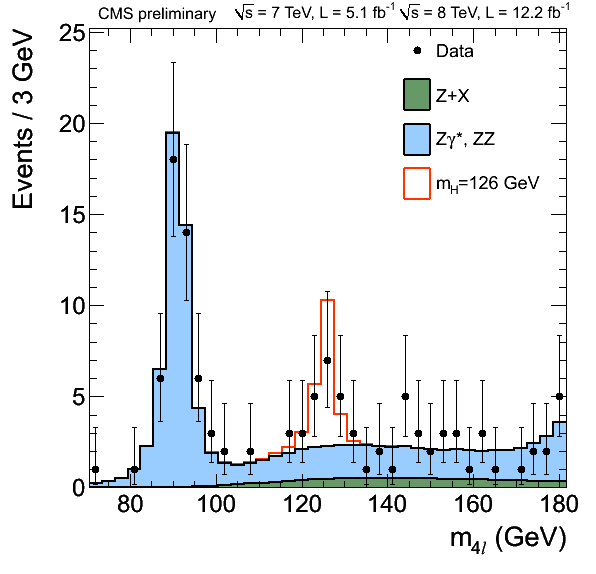
\includegraphics[width=3in]{figures/ZZMass_7Plus8TeV_70-180_3GeV.png}
\caption{4l invariant mass distribution showing H discovery in the ZZ* decay channel. The red line shows the signal distribution for $m_H=126$ GeV. Figure taken from https://twiki.cern.ch/twiki/bin/view/CMSPublic/Hig12041TWiki}
\label{4l}
\end{figure}


\section{Dark matter}


\subsection{Observational evidence}

\subsection{Beyond the Standard Model}

\subsubsection{Effective field theory}

\subsubsection{Simplified models}
